\subsection{Neo4j}

Ist eine Graph Datenbank die durch Beziehungen(Edges) aneinander gekoppelt werden und durch denn Typen(Label) Gruppiert werden können und so mit eine Abhängigkeit darstellen.
\\
Es wird erst ein Knoten-Typ bestimmt, der quasi sagt zu welcher Kategorie der Knoten gehört und dann die Eigenschaften(Property) in de ein Value als String oder integer ist, mann ist nicht auf eine Eigenschaft beschränkt.

\subsubsection{Beispiel}

\begin{verbatim}
create (l:Linux {challange:"Linux CLI", keyword:"cli", keyword:"linux"}) return l
\end{verbatim}

\begin{itemize}
    \item Wenn man dann zwei Challenge(Node´s) erstellt hat kann man sie mit einer Beziehung(Edge) verknüpfen in dem man:
\end{itemize}

\begin{verbatim}
create (l)-[:linux]->(l2)
create (l)<-[:linux]-(l2)
\end{verbatim}
\begin{itemize}
  \item Man könnte natürlich auch beim erstellen von Edges auch neue Propertys anlegen:
\end{itemize}

\begin{verbatim}
create (l)-[:linux{os:[Linux]}]->(l2)
\end{verbatim}

\subsubsection{Test-Graphmodell des STEMgraph-Projekts}

\subsubsection*{1. Datenmodell}

\begin{itemize}[itemsep=2pt]
  \item id: Identifizierung der Challenge
  \item teaches: Was wird gelehrt?
  \item depends\_on: Wovon hängt sie ab?
  \item keywords: Welche Themen sind vorhanden?
\end{itemize}

\subsubsection*{2. Testdaten und Beziehungen}

\begin{verbatim}
CREATE
(a:Challenge{
    uuid: "7392771207492170471730773974971", teaches: "Linux CLI Grundlagen",
    depends_on: [], keywords: ["ClI", "Linux"]
}),
(b:Challenge{
    uuid: "27498625678403678296478352674894", teaches: "Dateien und Ordner verwalten",
    depends_on: ["7392771207492170471730773974971"], keywords: ["files", "linux"]
}),
(c:Challenge{
    uuid: "23684937628947256748937849374783", teaches: "Makefile Grundlagen",
    depends_on: ["27498625678403678296478352674894"], keywords: ["makefile", "build"]
}),
(b)-[:BUILDS_ON]->(a),
(c)-[:BUILDS_ON]->(b)
\end{verbatim}

\subsubsection*{3. Graph-Datenbank View}

\begin{figure}[htbp]
  \centering
  \begin{minipage}[b]{0.45\textwidth}
    \centering
    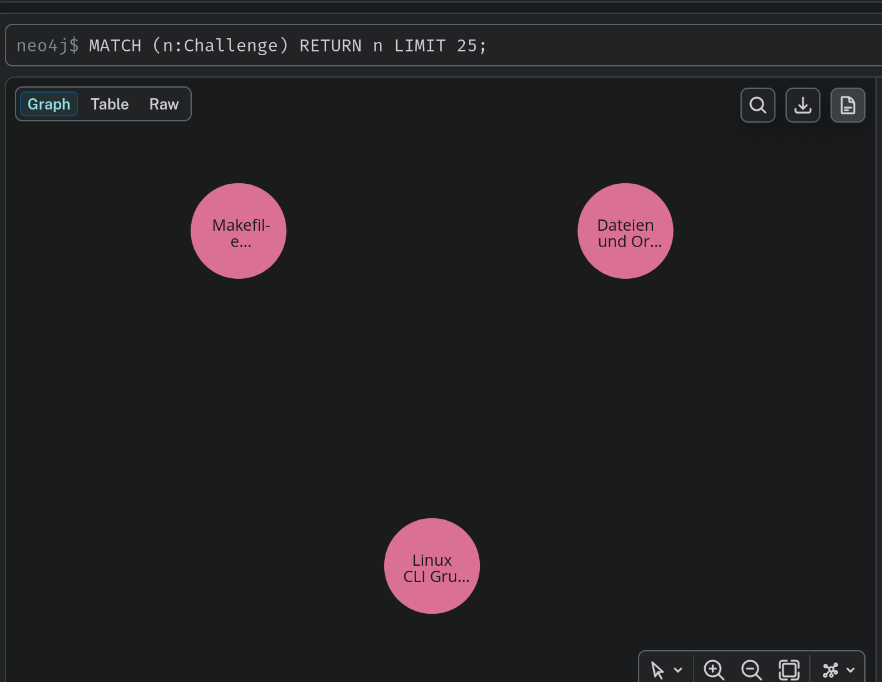
\includegraphics[width=6cm]{Bilder/Neo4j_Challenges.jpg}
    \caption{Challenges}
    \label{fig:bild1}
  \end{minipage}
  \hfill % Fügt automatisch den maximalen Abstand zwischen den Bildern ein
  \begin{minipage}[b]{0.45\textwidth}
    \centering
    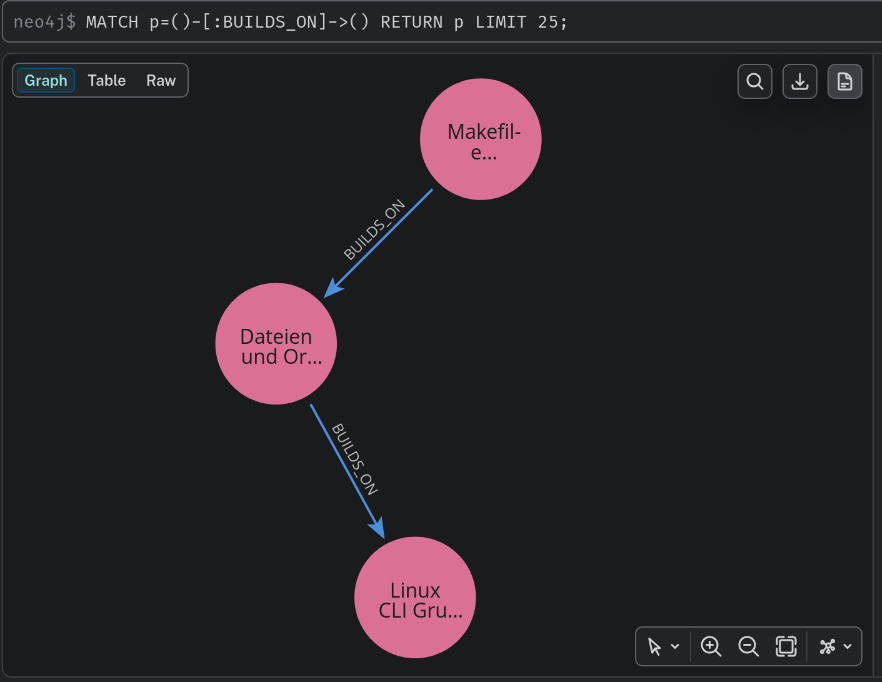
\includegraphics[width=6cm]{Bilder/Neo4j_Abhängigkeiten.jpg}
    \caption{Challenges mit Abhängigkeiten}
    \label{fig:bild2}
  \end{minipage}
\end{figure}

\subsubsection*{4. Neo4j Test}

Hab die ersten Test \texttt{Challenge}-Knoten angelegt und abgefragt. Dabei habe ich drei Challenges \texttt{Linux CLI Grundlagen}, \texttt{Dateien und Ordner verwalten} und \texttt{Makefile Grundlagen} als Knoten angezeigt.
\\
Danach habe ich die Beziehungen mit \texttt{BUILDS\_ON} geprüft. Es zeigt, dass \texttt{Makefile Grundlagen} auf \texttt{Dateien und Ordner verwalten} aufbaut und \texttt{Dateien und Ordner verwalten} wiederum auf \texttt{Linux CLI Grundlagen} verweist.
